\documentclass[10pt, letterpaper, twoside]{article}

\usepackage{epsfig}
\usepackage{verbatim}

\author{Conor McGann, Tania Bedrax-Weiss, Andrew Bachmann}

\title{PLASMA 1.0: User Guide}

\begin{document}

\maketitle

\section{Introduction}
PLASMA ({\bf PLA}n {\bf S}tate {\bf M}nagement {\bf A}rchitecture) is a component-based software library for representation and reasoning with plans within a constraint-based paradigm. Our goal in developing PLASMA is to provide a fast, flexible, extensible, reusable technology platform for building planning and scheduling applications suitable for space exploration. PLASMA is derived from EUROPA [] which has been the core planning technology for a variety of NASA-relevant research and mission application. A notable example is  MAPGEN [], the ground-based daily activity planning system for the Mars Exploration Rover mission. EUROPA in turn is derived from HSTS [] which was the planner for the Remote Agent[]. PLASMA builds on the legacies of EUROPA and HSTS in its support for constraint-based temporal-planning techniques. However, it provides a richer modeling language, and a highly modular and extendible architecture which has resulted in improved performance and opened the technology to a broader range of planning techniques (e.g. POCL planning). 

The philosophy underlying PLASMA is to acknowledge up front that no one size fits all when it comes to which techniques to use, and which capabilities to employ. Consequently, PLASMA is engineered to allow people to take just what they need, discard what they do not, and integrate extensions to suit their particular requirements in a straighforward manner. The design strategy is to focus on a core framework defininig the principal abstractions and interactins induced by our underlying paradigm. We then provide concrete components to allow particular assemblies to be defined. With this component-based framework we have strived to strike a balance between flexibility and efficiency.

The content of this guide is laid out as follows. We begin with an explanation of the concepts underlying PLASMA addressing its role as an embedded technology within a planner, and its underlying paradigms for representation and reasoning. We then switch gears to get the reader up and running with a particular assembly of PLASMA that is included with the distribution. In this section, the reader will solve a prepared planning problem with PLASMA, without really understanding much about how it happened! Following this, we seek to build up some understanding with a tutorial-like exposition of model development, and problem solving with PLASMA's primary modeling language - NDDL. Having spent some effort working on the application of PLASMA, we turn to its underlying architecture. This section gets 'under-the-hood' to provide an understanding of how PLASMA works at the implementation level.  Finally, we address the technical aspects of customization and extension. Detailed reference material is included in the appendices.

\section{Concepts}
\subsection{Plans in Planning, Scheduling and Execution}
Explain the notion of a {\em Plan} as a central representation of state that is used in planning, scheduling and execution. Give examples. Pose the common problem in terms of a partial plan that must be evolved to be correct and complete for the purposes of the user of the plan. Discuss each type of task in terms of their impact on a Plan.
\subsection{Plan Representation}
\subsubsection{Time-dependent state and action}
Talk about Objects that have state and behavior that are temporally qualified. Object state and behaviour can be described by predicates with temporal Extent. Objects with state that is not temporally qualified is a special case where the extent of the behavior is infinite.
\subsubsection{Flexibility}
Introduce the notion of flexibility, why it is necessary. This is based on the principle of least commitment and lack of precise knowledge. Then show a mapping to variables.
\subsection{Plan Entities and Relationships}
The Entities are first and foremost Object, Token, Variable. Since we have to concern ourselves with relationships among entities in the plan, we need to also introduce the idea of Constraints. Draw a diagram indicating the core entities and their relationships. Indicate how these relationships are encaptured through the use of constraints. We should be sure to have introduced the Token state model.
\subsection{Plan State Management}
Now we want to address the desire to assure completeness and correctness. Infrastructure can be built in to leverage the representation in order to assure these properties. We can thus talk about the automated reasonining capabilities that can be used to propagate consequences (changes to variable values, introduction of sub-goals and ocnstraints), as well as test for consistency.

\section{Hello Rover - Getting started with PLASMA}
Should demonstrate a simple example that takes an initial state, a model, and runs them through the planner. Will generate output and display output in PlanWorks to visualize the plan. This should illustrate the round trip through the process. Will be a fairly brief section, but should address issues of running the planner, point out the particular examples to draw from. Reference PlanWorks if it is available, and indicate how it can be used to visualize the plan. The products of this section when the user is done will be \verb!model.nddl, initial-state.nddl, Jamfile, ppw_config.!

\subsection{Creating a Project}
This should reference the script, and talk about what is created by the script for your project.
\subsection{Building a simple model}
\subsection{Creating an initial state}
\subsection{Running the planner}
Include setting up the Jamfile for the planner run, with the model and initial states. Also include setting up the ppw-config file.
\subsection{Visualization of the plan and planning process in PlanWorks}
We will not go into all the details. Refer to PlanWorks documentation for setup instructions of use. We may wish to include screen shots.

\section{Model Development}
For the purposes of this section, we will assume the application is a planning task, and that we can use the built in CBPlanner in PLASMA.
This is where we get through all the modeling. Should take it through as a tutorial, which will be accompanied by examples that can be run. We can use the example of the K9 model from the Contingent Planning Team to motivate the problem, since they have pushed alot of the modeling features.

\subsection{Rover: The Robotic Geologist}
Rover is 6 wheeled robot equiped with a range of instruments to sample and study a geological site. Rover will process goals for taking pictures and rock samples in various locations within a given survey area. It has on board a battery, and can replensih its energy levels using solar power. Rover is also equiped with communication equipment allowing it to send and receive data to and from mission control. Our Rover is a fictitous creature. Our goal in model development is to develop a model of Rover which will allow plans to be developed to meet mission goals expressed in high-level terms, such as:
\begin{enumerate}
\item Take a panoramic image at position p, time t, and orientation o.
\item Take a rock sample of rock r.
\item Take a soil sample at position p.
\end{enumerate}

In fulfilling these objectives, goals must be mapped to command sequences to Rover's control subsystem. Rover includes a number of components that can be operating concurrently. For example, the Camera can be tracking targets while Rover is driving. Conversely, Rover may require that certain components are in certain states while other components are in other states. For example, the rock abrasion tool must be stowed while Rover is moving. We must also address sequencing rules within a component. For example, in order to take a sample of a rock, the sampling instrument must be position at a precise location a few millimetres from the rock surface. Prior to being in such a position, the uinstrument must be first unstowed, and then positioned. Our model must include these interactions within a component and among components so that the planning process can devise command sequences to achieve the mission goals and {\em cannot} produce incorrect command sequences.

\subsection{Basic navigation}
Many of the goals which Rover may be tasked with require mobility. Specifically, Rover must navigate from one location to another in a given site area without bumping into anything, and without getting into other difficulties such as running out of energy. For our purposes, we will start by focussing on a simplified version of the navigation problem. We will assume that the site of operation is represented by a grid of X and Y co-ordinates (integers). A location is thus a position in this grid. Rover may be at a location, or going from one location to another. We will ignore otherwise important details such as obstacle avoidance and resource management.

\subsubsection{Representing the site}

\subsubsection{Rover state and action}

\subsubsection{Constraining interactions}

\subsubsection{Going from Lander to Rock}

\subsubsection{Formulate and solve the planning problem}

\subsubsection{Recap}
We should have covered:
\begin{enumerate}
\item class
\item enum
\item float, int, string
\item inheritance
\item predicates
\item predicate parameter constraints
\item basic rules - meets and met\_by
\item instantiation
\item assigment
\end{enumerate}

\subsection{Turning goals into reality - taking a picture}

\subsubsection{Recap}
We should have covered:
\begin{enumerate}
\item composition
\item contains/containedBy
\item enum
\item float, int, string
\item composition
\item inheritance
\item predicates
\item predicate parameter constraints
\item basic rules - meets and met\_by
\item instantiation
\item assigment
\end{enumerate}

\subsection{Handling relationships between predicates and variables}
\subsubsection{Recap}
We should have covered
\begin{enumerate}
\item Constraints among parameters of a predicate.
\item Rules
\item Allen Relations
\end{enumerate}
End the section by referencing a model and initial state that can be run through the planner and visualized in PlanWorks.

\subsection{Advanced rule writing}
\subsubsection{Recap}
We should have covered:
\begin{enumerate}
\item local variables
\item guards
\item object reference model
\item existential quantification
\item universal quantification
\item macros
\item additional allen relations
\end{enumerate}
End the section by referencing a model and initial state that can be run through the planner and visualized in PlanWorks.

\subsection{Incorporating resources}
\subsubsection{Recap}
We should have covered:
\begin{enumerate}
\item The details of the built in base class. 
\item How one can define ones own resource.
\item Example illustrating use of the constructor.
\item Example illustrating simple case of production and consumption.
\item Example illustrating discretization into events.
\item Careful explanation of the issue of closure and bounding of the resource.
\end{enumerate}

End the section by referencing a model and initial state that can be run through the planner and visualized in PlanWorks.

\section{PLASMA System Architecture}

\begin{figure}[t]
\centering\epsfig{file=SystemDiagram.eps, width = 3.25in}
\caption{PLASMA system architecture diagram}
\label{SystemDiagram}
\end{figure}

Picture of overall architecture. Document each component at the level of its main roles and responsibilities. This should be used as an introduction to the API documentation. Ideally, we could directly leverage that documentation.
\subsection{Plan Database}
\subsection{Constraint Engine}
\subsection{Temporal Network}
\subsection{Rules Engine}
\subsection{Resources}
\subsection{NDDL Parser and Compiler}
\subsection{Utilities}
\subsection{CBPlanner}
\subsection{Key use cases}


\begin{figure}[t]
\centering\epsfig{file=TokenStateModel.eps, width = 3.25in}
\caption{Token State Transition Diagram}
\label{TokenStateModel}
\end{figure}


Helps to understand the interaction among components. May want to use a simple example model, possibly cut-down from k9.
\begin{enumerate}
\item Creating an Object
\item Token activation
\item Token deactivation
\item Constraining a Token
\item Freeing a Token
\item Binding a Variable
\item Freeing a Variable
\item Copying a plan database
\end{enumerate}

\section{Customization and Extension}
\subsection{Configuration and Assembly}
\subsection{Using and extending the CBPlanner}
\subsection{Custom constraints}
\subsection{Custom propagation}
\subsection{Building model specializations}
\subsection{Custom rule implementations}
\subsection{Specialized domains}
\subsection{External data integration}
\subsection{Listeners and Loggers}
\subsection{Integration to PlanWorks}

\section{Bibliography}

\section{Appendices}
\subsection{Appendix A: NDDL Language Reference}
class
predicate
int
float
string
enum
extends
before
after
contains
contained_by
meets
met_by
concurrent
precedes
object
start
end
duration
state
time
any
new
goal
rejectable
activate
specify
constrain
close

\subsection{Appendix B: Constraint Library Reference}
\subsection{Appendix C: Test Language Specification and Use}
\end{document}



